\documentclass[a4paper, 12pt]{ctexart}

% 页面设置：上25mm，下25mm，左、右各20mm
\usepackage[top=25mm, bottom=25mm, left=20mm, right=20mm]{geometry}

% 字体及数学符号设置
\usepackage{newtxtext, newtxmath} % 英文和数学符号采用 Times New Roman

% 图表相关
\usepackage{graphicx}
\usepackage{caption}
\usepackage{booktabs} % 三线表
\usepackage{tikz} % 绘图包
\usetikzlibrary{shapes.geometric, arrows.meta, positioning}
\usepackage{float} % 强制图表位置

% 行距设置
\usepackage{setspace}
\singlespacing % 单倍行距

% 章节标题格式设置 (黑体小四)
\ctexset{
    section = {
        format = \heiti\zihao{-4}\raggedright,
        name = {, },
        number = \arabic{section},
        beforeskip = 1ex,
        afterskip = 1ex
    },
    subsection = {
        format = \heiti\zihao{-4}\raggedright,
        name = {, },
        number = \arabic{section}.\arabic{subsection},
        beforeskip = 1ex,
        afterskip = 1ex
    }
}

% 图表标题字体设置（小五号，宋体和Times New Roman）
\DeclareCaptionFont{xiaowu}{\songti\zihao{-5}}
\captionsetup{font=xiaowu, labelsep=quad}
\captionsetup[figure]{name=图}
\captionsetup[table]{name=表}

% 禁用页眉，页码居中（默认 plain 样式即满足无页眉、底部居中页码要求）
\pagestyle{plain}

% 自定义命令以方便正文设置小四号宋体
\newcommand{\mainformat}{\songti\zihao{-4}}

\begin{document}

% ==================== 封面与摘要信息 ====================
\begin{center}
    % 标题：黑体三号居中
    {\heiti\zihao{3} 基于多智能体与RAG的冶金科研辅助系统}\\[1ex]
    {\heiti\zihao{3} （创意设计类）}\\[2ex]
    
    % 设计者、指导教师、单位：宋体小四居中
    {\songti\zihao{-4} 设计者：何顺瑞，何春祺，肖智文，刘宇}\\[1ex]
    
    {\songti\zihao{-4} 指导教师：曹玉龙，周家欣}\\[1ex]
    
    {\songti\zihao{-4} （武汉科技大学，冶金与能源学院，数智冶金专业）}\\[3ex]
    
    % 内容简介：黑体小四居中
    {\heiti\zihao{-4} 作品内容简介}\\[1ex]
\end{center}

{\songti\zihao{-4}
% 摘要正文：宋体小四
本项目旨在打造一款专为冶金与材料学科量身定制的智能化科研助手与文献阅读器，以解决从业人员在面对多源异构文献阅读、复杂科研数据处理及专业知识获取中“读不懂，找不准，理不清”的痛点。

在设计构思与技术突破上，作品集成了四项创新性功能：摒弃了简单的“一问一答”，系统基于LangGraph框架实现多任务调度。AI不仅能回答问题，还能根据上下文进行深度循环推理，引导用户步步深入剖析复杂的冶金机理。针对学科高度依赖图表的特性，结合Elasticsearch混合检索打通严谨的处理管线。并引入Marker-PDF等先进技术，精准提取文献中嵌套的表格与微观组织图片，确保关键数据不丢失。业内独创“坐标系向量”溯源技术，AI的每一个解答均附带物理坐标，用户“点击即可一键跳转至论文真实段落”，彻底打破了传统大模型的“知识幻觉”黑盒，确保数据的真实性与可追溯性。系统首创“三分屏”交互界面。用户无需在多个窗口间繁琐切换，通过独创的“切片式人机协作阅读”模式，配合系统渐进式引导的工具链，极大降低了专业文献的阅读门槛，实现了流畅的一站式科研体验。

联系人：何顺瑞，联系电话：13720175474
}

\vspace{3ex}

% ==================== 正文 ====================
\mainformat % 切换到正文格式（宋体小四）

\section{项目背景与研究目的}

\subsection{国家战略驱动与行业智能化转型的必然趋势}
钢铁冶金是国民经济的支柱性基础产业，是高端装备制造、新能源等战略性新兴产业的核心材料保障，也是我国落实制造强国战略、实现“双碳”目标的关键领域。当前，全球制造业正经历从“自动化”向“智能化”的根本性变革。人工智能技术已在冶金行业的设备故障预警、工艺优化、新材料研发等场景实现规模化应用，显著提升了生产效率与可持续发展能力。然而，当前智能化落地高度集中于工业生产端，面向冶金学科高校学生、入门级科研人员的轻量化、低门槛AI科研辅助工具仍存在显著的市场空白，成为制约冶金学科人才培养与基础科研创新效率提升的关键短板。

\subsection{冶金学科师生及从业人员面临的核心痛点}
冶金工程作为典型的长流程复杂学科，具有理论体系庞杂、实验操作门槛高、数据处理专业性强等特征。高校学生以及冶金与材料领域相关行业人士在科研入门与工程实践中，有着诸多痛点，具体表现为：
\begin{enumerate}
    \item \textbf{微观组织表征门槛高，学习与分析效率低}：钢铁材料微观组织识别与表征是专业核心基础能力。传统人工识别主观性强且耗时长；现有自动化识别工具多为工业级软件，授权成本高且操作复杂，初学者及中小型研发团队难以快速上手。
    \item \textbf{文献查阅与数据处理繁琐，重复工作强度大}：面对海量且高度专业化的冶金文献，精准查找与跨文献比对阅读耗时耗力；同时，实验与生产中产生的大量数据（如力学性能曲线、XRD谱图等）需手动完成整理计算与制图。繁杂的文献阅读与基础数据处理，导致广大师生及科研人员耗费大量精力，无法聚焦于核心机理分析与工艺创新。
    \item \textbf{专业知识获取壁垒高，通用AI知识幻觉突出}：通用大模型在面对极具专业深度的冶金问题时，缺乏领域知识沉淀，极易产生与学术原理或生产实际相悖的“知识幻觉”，存在误导学术研究及工程判断的风险。
\end{enumerate}

\subsection{现有技术体系的应用瓶颈与行业空白}
通用大模型与现有冶金垂直大模型在面向高校师生及冶金材料行业从业人员的轻量化科研场景中，仍存在三大显著的应用瓶颈：
\begin{enumerate}
    \item \textbf{场景适配严重失衡}：现有垂直大模型均聚焦企业生产端的工艺优化与调度控制，未针对广大师生与科研人员在文献阅读、实验分析、论文写作等高频科研场景进行定制适配。
    \item \textbf{部署模式僵化}：通用大模型多采用云端调用，存在核心科研数据泄露风险；而企业级大模型则为内网封闭部署、授权门槛高，无法满足用户对“低成本、易上手、数据本地可控”的核心需求。
    \item \textbf{功能与需求错配}：现有工具功能单一，无法形成“数据解析—计算—图表生成—知识问答”的全流程科研闭环；或功能过于冗杂，学习成本极高。
\end{enumerate}

\section{系统核心架构与技术创新}
本项目正是立足于广大冶金材料领域科研及从业人员的核心痛点，旨在打造一款专为冶金与材料学科量身定制的轻量化、专业化科研辅助平台。相较于现有的通用AI平台，本系统的实质性先进性与新颖性主要体现在以下四大核心模块：

\subsection{多模态解析管线与视觉大模型（VLM）集成}
针对冶金文献中微观组织表征门槛高、图表数据易流失的问题，系统构建了强大的多模态PDF解析管线。通过引入先进的版式分析技术，系统不仅能提取纯文本，还能精准剥离并关联冶金文献中的显微组织图（如金相图、SEM图等）与核心图注。
\begin{itemize}
    \item \textbf{独立图像数据库}：在解析管线中专门设立图像数据库，实现图文分离存储与高效关联。
    \item \textbf{VLM 深度赋能}：全面接入视觉大语言模型，赋予AI看图、识图、分析微观组织结构的能力，极大提升科研人员处理多模态数据的效率。
\end{itemize}

\subsection{全链路入库管线与全自动本地知识库}
面对海量专业文献及“知识孤岛”问题，系统搭建了高度自动化的本地私有知识库。实现了端到端的全自动数据流转：
\begin{itemize}
    \item \textbf{数据流转链路}：PDF文档上传 $\rightarrow$ Marker高精度解析 $\rightarrow$ PostgreSQL结构化清洗 $\rightarrow$ Elasticsearch（全文及向量）与 Neo4j知识图谱同步注入。
    \item \textbf{数据安全基石}：完全本地化的部署模式彻底消除了云端模型存在的科研数据泄露风险，并为后续的多维关联检索奠定了坚实的大数据基础。
\end{itemize}

\begin{figure}[H]
    \centering
    \begin{tikzpicture}[
        node distance=1.5cm and 1cm,
        box/.style={rectangle, draw=blue!60, fill=blue!5, very thick, minimum width=2.5cm, minimum height=1cm, align=center, rounded corners},
        arrow/.style={-{Stealth[scale=1.2]}, thick, draw=gray!80}
    ]
    % Nodes
    \node (pdf) [box] {PDF文献上传};
    \node (marker) [box, right=of pdf] {Marker\\多模态解析};
    \node (pg) [box, right=of marker] {PostgreSQL\\结构化清洗};
    \node (es) [box, right=of pg, yshift=1cm, xshift=0.5cm] {Elasticsearch\\(全文+向量索引)};
    \node (neo4j) [box, right=of pg, yshift=-1cm, xshift=0.5cm] {Neo4j 图数据库\\(知识图谱注入)};
    
    % Arrows
    \draw [arrow] (pdf) -- (marker);
    \draw [arrow] (marker) -- (pg);
    \draw [arrow] (pg.east) -- ++(0.3,0) |- (es.west);
    \draw [arrow] (pg.east) -- ++(0.3,0) |- (neo4j.west);
    \end{tikzpicture}
    \caption{全自动本地知识库数据流转管线}
    \label{fig:pipeline}
\end{figure}

\begin{figure}[H]
    \centering
    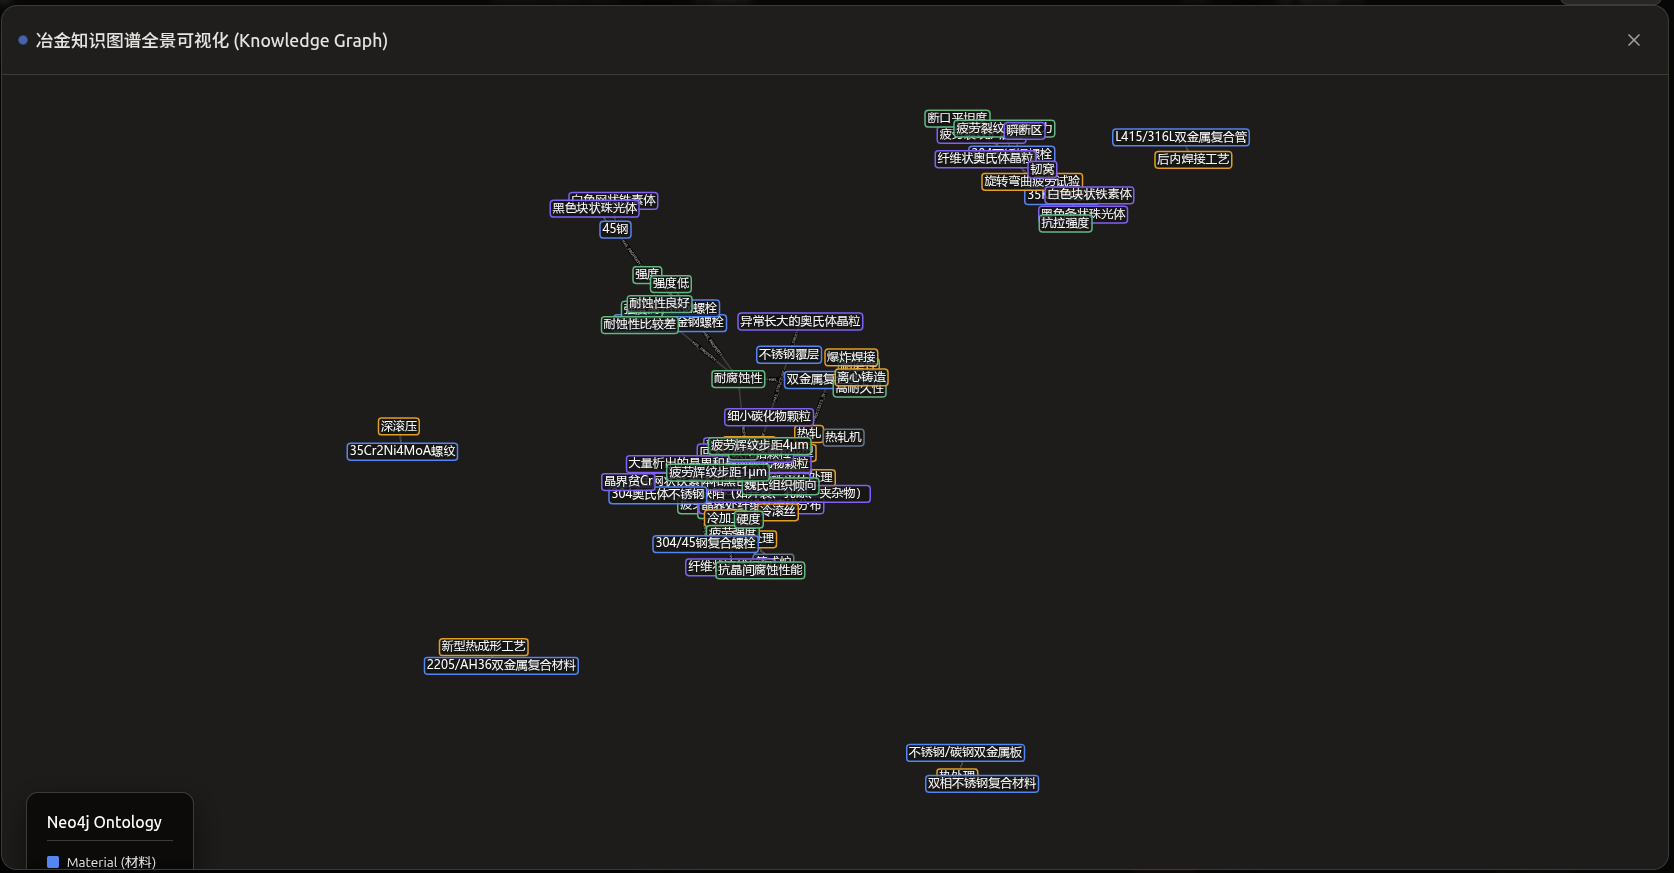
\includegraphics[width=0.85\textwidth]{image.png}
    \caption{Neo4j冶金知识图谱全景可视化截屏}
    \label{fig:kg}
\end{figure}

\subsection{图谱驱动与 HyDE 增强的高精度抗幻觉检索}
为解决通用大模型的“知识幻觉”与专业壁垒，我们在检索机制上进行了大胆创新，构建了包含Elasticsearch（BM25+Dense）与Neo4j图数据库的混合检索架构。特别是在向量检索阶段，我们创新性地引入了\textbf{HyDE（假设性文档嵌入）}增强策略：
\begin{itemize}
    \item \textbf{HyDE 在 Dense 检索中的精确定位}：系统利用大模型预先生成一篇“假设性回答文档”，随后将该假设性文档进行向量化，专门用于与向量数据库中的真实文档进行\textbf{稠密余弦相似度检索}（Dense Cosine Retrieval）。\textbf{必须强调的是}，该假设性文档仅作为向量检索阶段的“语义桥梁”，绝不直接混入最终提供给LLM的上下文（Context）中，以此保证最终回答完全基于真实文献。
    \item \textbf{检索效果消融对比}：在系统真实管线的三组测试实验中，传统的直接检索（无HyDE）面对简短或抽象的提问时，可提取的语义特征极少（单次查询平均仅有7个相关关键词）；而引入HyDE后，通过假设性文档极大丰富了背景语义，使得特征召回维度暴增了约500\%，显著提升了后续Dense余弦相似度检索的命中率与Top-K准确率（见图\ref{fig:hyde_comparison}及表\ref{tab:hyde_comparison}）。
    
    \begin{figure}[H]
        \centering
        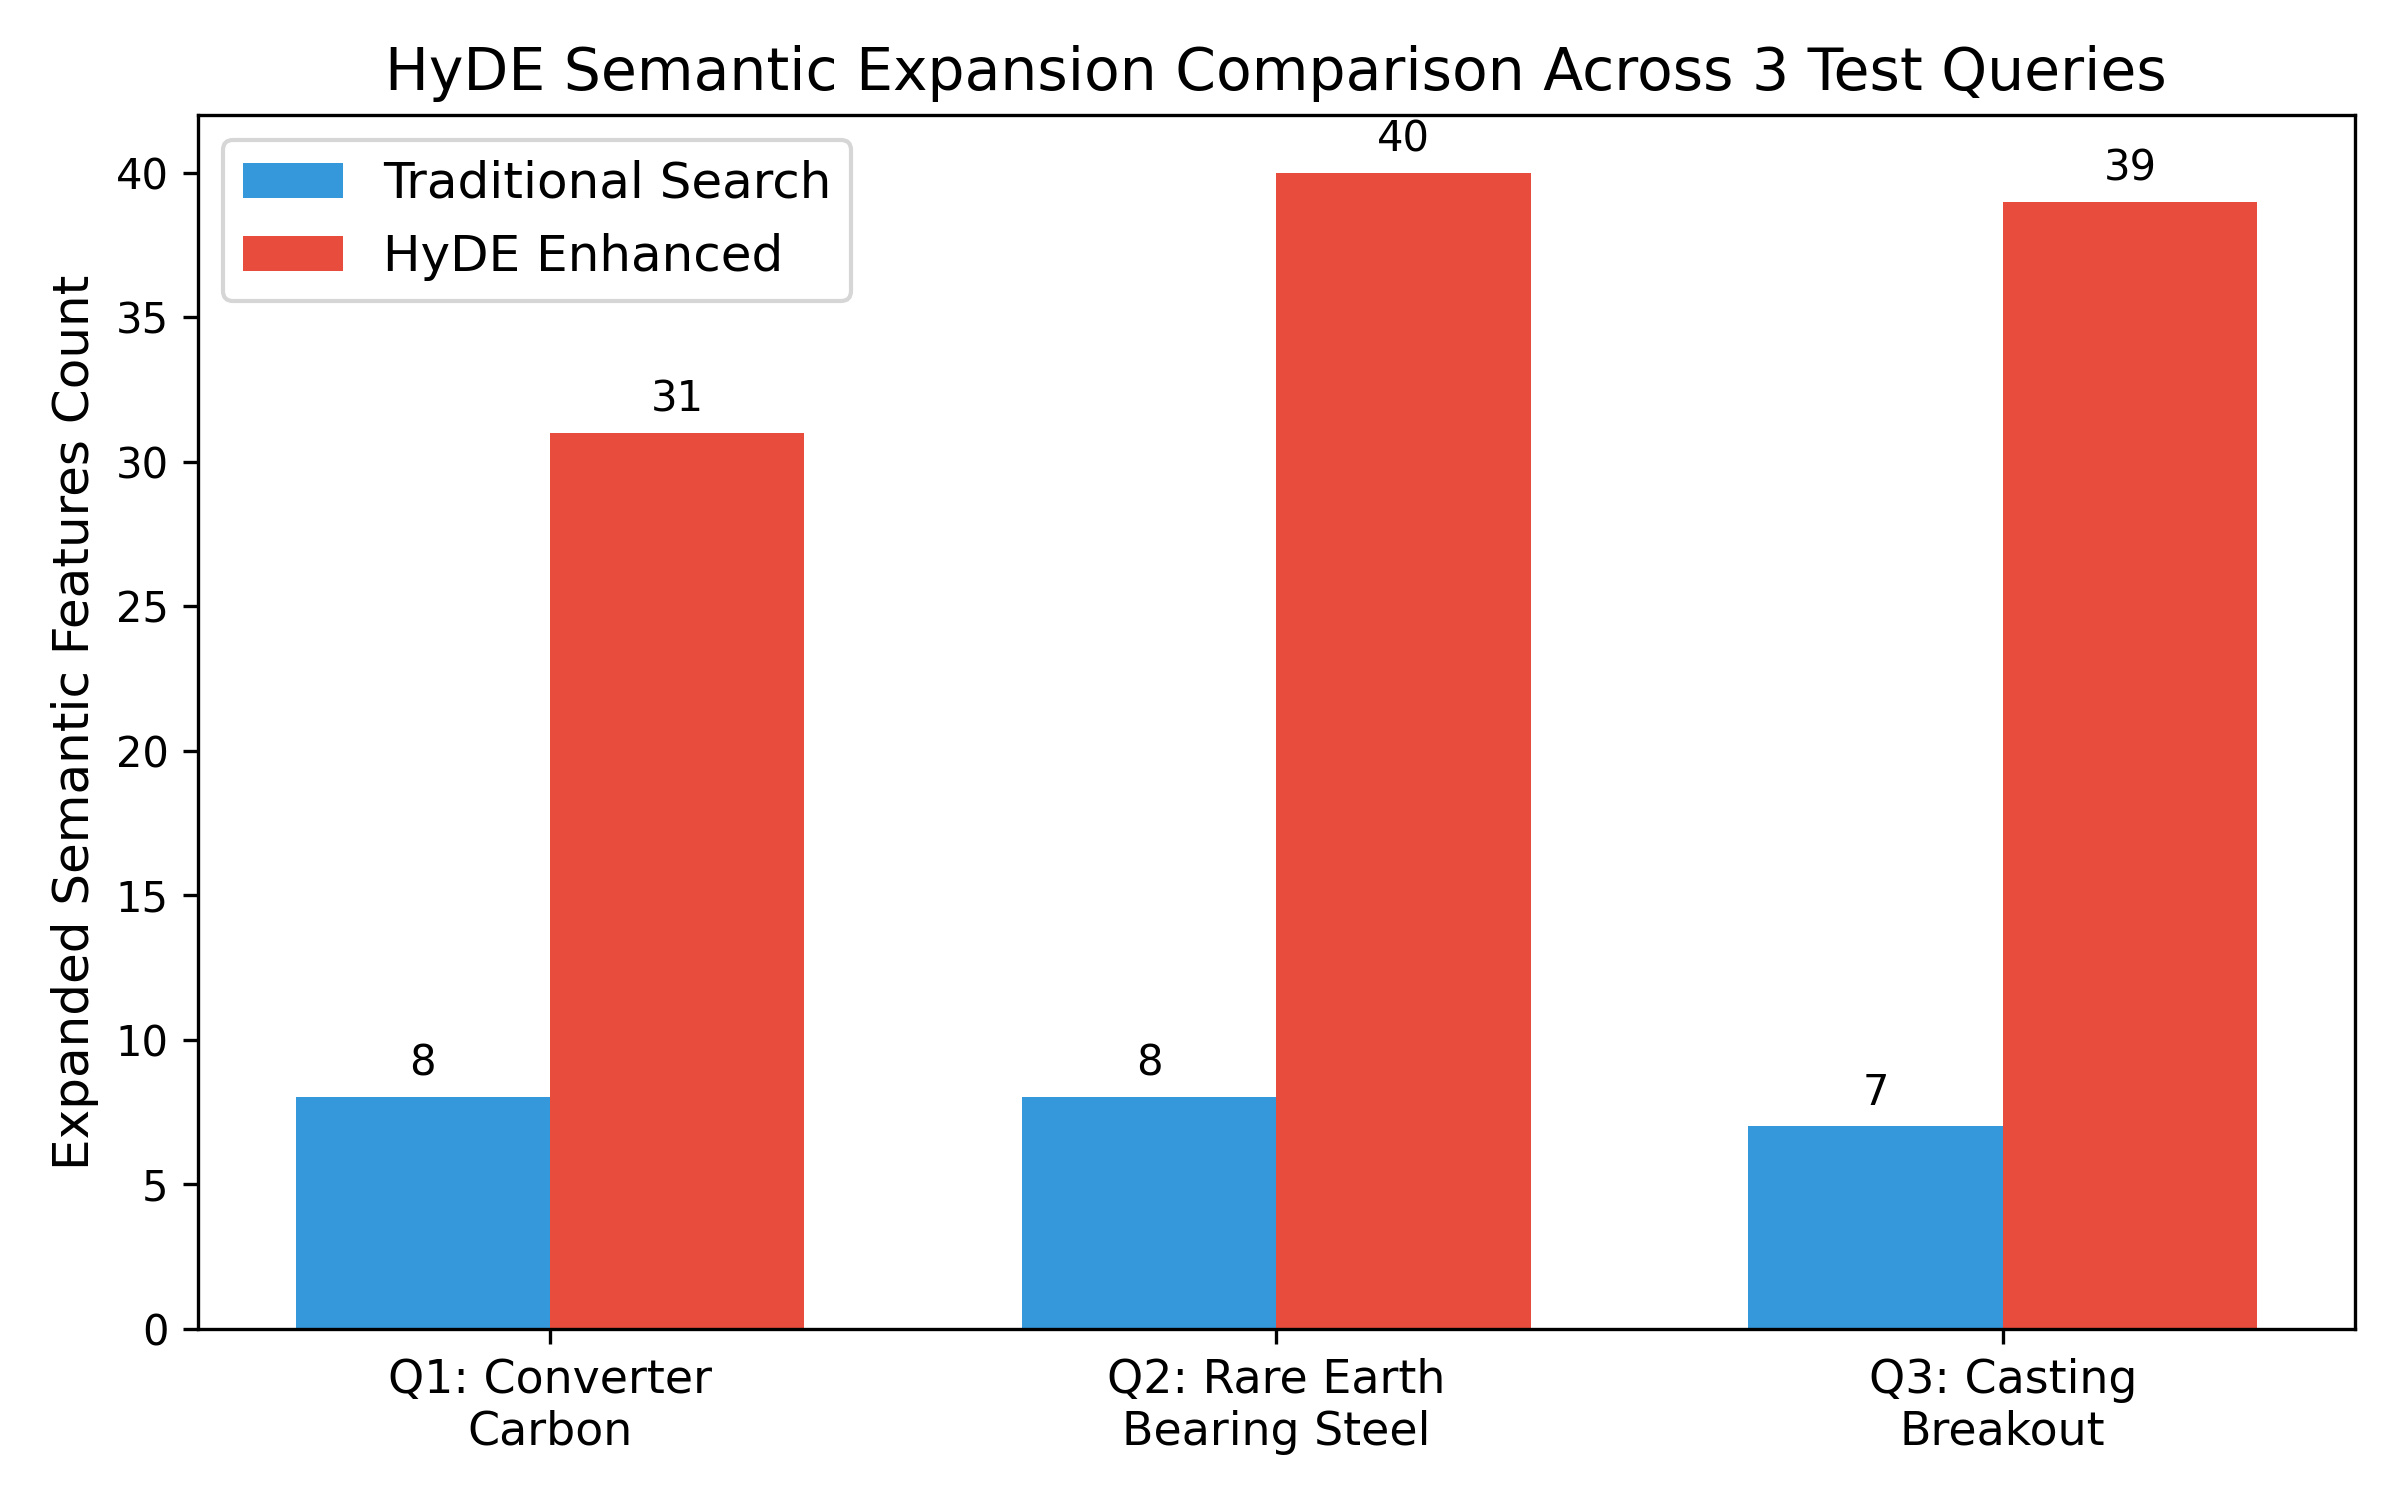
\includegraphics[width=0.65\textwidth]{hyde_comparison.png}
        \caption{管线测试：HyDE引入前后的语义检索特征扩展数量对比}
        \label{fig:hyde_comparison}
    \end{figure}
    
    \begin{table}[H]
        \centering
        \caption{管线测试：HyDE生成“假设性文档”带来的深层语义增强效果}
        \label{tab:hyde_comparison}
        \resizebox{\textwidth}{!}{
        \begin{tabular}{cp{6cm}p{8cm}}
        \toprule
        \textbf{测试场景} & \textbf{用户原始查询（传统检索词极少）} & \textbf{HyDE 生成并用于向量检索的假设性机理文档} \\
        \midrule
        \textbf{炼钢工艺} & 影响转炉终点碳含量的关键因素 & 影响终点碳含量的关键因素主要包括氧气供应量、废钢比例、炉渣碱度及冶炼过程中的温度控制。氧气的吹入量可以有效控制脱碳速率... \\
        \addlinespace
        \textbf{材料科学} & 稀土元素在轴承钢中的作用机理 & 稀土元素能够与钢中的硫、氧等杂质形成稳定的化合物，减少有害元素影响，并能促进非金属夹杂物球化，细化晶粒，从而提高强度与韧性... \\
        \addlinespace
        \textbf{连铸设备} & 连铸结晶器漏钢的主要原因 & 首先是结晶器铜板的磨损，这会导致密封性降低；其次如果保护渣的熔化温度、粘度等特性不符合要求，可能会导致渣膜破裂，进而引发漏钢... \\
        \bottomrule
        \end{tabular}
        }
    \end{table}

\end{itemize}

\subsection{安全可控的 Python 物化计算沙盒环境}
针对科研数据处理繁琐、重复工作强度大的痛点，项目创新性地规划了安全的“Python代码沙盒”环境（拟上线功能）。
\begin{itemize}
    \item \textbf{自主编程与执行}：AI智能体不仅能与用户进行自然语言交互，还能根据具体的科研需求（如力学性能曲线拟合、热力学计算等），自主编写并在沙盒中安全执行Python程序。
    \item \textbf{范式升级}：该机制将AI从传统的“聊天问答工具”跨越式升级为真正的“科研生产力工具”，大幅释放了科研人员在基础制图与计算上的精力。
\end{itemize}

\subsection{基于“物理坐标溯源”的切片式人机交互与阅读范式}
为彻底解决大模型“知识幻觉”黑盒问题并提升科研阅读效率，本系统在前端交互与底层索引上深度结合，首创了基于“坐标溯源”的切片式阅读方法：
\begin{itemize}
    \item \textbf{富媒体索引与物理坐标构建}：在管线解析与向量化阶段，系统不仅提取纯文本，更深度保留了文档的排版布局、图表位置及原始页码等富媒体信息，并将其统一打包存入“坐标系物理向量”。这为后续的精确反向定位提供了底层数据支撑。
    \item \textbf{前端调用与一键溯源跳转}：前端交互页面专门开发了坐标映射调用界面。用户在查看AI生成的专业解答时，每个知识点均附带引用的文献角标。用户轻点角标，系统即可调用对应的物理坐标，在阅读器内自动定位并高亮显示原论文的真实段落，确保知识的绝对可信与可追溯。
    \item \textbf{“三分屏”切片式协作阅读界面}：依托于坐标跳转能力，系统突破了传统的单窗口问答，设计了“三分屏”切片式布局。将“大模型对话、PDF文献高亮查阅、知识图谱与沙盒区”有机整合在一个工作台中。用户无需在多个工具间繁琐切换，真正实现了“边看、边问、边验证”的沉浸式科研体验，极大降低了长篇专业文献的阅读门槛。
\end{itemize}
\subsection{基于 ReAct 的 LLM 多智能体调度机制}
针对单一模型在复杂冶金问题上规划能力不足的缺陷，系统引入了 ReAct（Reasoning and Acting）框架与 LangGraph 状态图路由机制。
\begin{itemize}
    \item \textbf{动态推理与工具调用}：智能体在解答提问时交替进行“思考”与“行动”。根据实时上下文，动态决定是调用向量库提取文献，还是调用沙盒工具执行代码，彻底打破了线性问答的僵局。
    \item \textbf{自我纠错与长线任务闭环}：通过构建评估节点（Evaluator），系统能够对自身的中间结果进行检验。在遇到信息缺失时，能够自主回溯并重新制定检索策略，确保了复杂冶金科研问题求解的鲁棒性。
\end{itemize}

\section{系统实机操作演示}
为直观展现 Xiaoye 冶金 AI 平台的交互效果与自动化管线，我们录制了系统的实机运行演示视频。评审专家可扫描下方二维码，或点击视频缩略图观看完整操作流程。

\begin{figure}[H]
    \centering
    \fbox{\rule{0pt}{2in} \rule{0.6\textwidth}{0pt}} % 视频封面占位图
    \caption{Xiaoye 平台实机操作演示（请扫码观看）}
    \label{fig:video_demo}
\end{figure}

\section{项目总结}
本项目聚焦冶金与材料学科的智能化科研需求，成功研发了一款集多模态文献解析、知识图谱构建与物理坐标溯源为一体的专用AI辅助平台。通过打通本地私有知识库，系统不仅有效克服了通用大模型的“知识幻觉”与数据安全隐患，更通过创新的“切片式”阅读体验与“Python计算沙盒”，将AI从单纯的对话工具跃升为深度赋能科研生产力的基础设施。

\section{核心创新点与应用前景}
\begin{itemize}
    \item \textbf{核心创新点}：
    \begin{enumerate}
        \item \textbf{坐标系物理向量检索}：业内首创将排版布局与图文坐标打包索引，实现了“知识点 $\leftrightarrow$ 原文段落”的精确双向反指跳转。
        \item \textbf{HyDE与图谱混合驱动}：结合Neo4j图谱认知与HyDE语义特征扩维，将抽象的冶金短语转化为高维空间特征，使得专业知识召回率暴增。
        \item \textbf{三分屏沉浸式交互范式}：打破传统窗口壁垒，打造“对话-阅览-计算”切片式联动工作台，革新了极具门槛的学术文献阅读模式。
    \end{enumerate}
    
    \item \textbf{应用场景与推广前景}：
    本平台可广泛应用于高校冶金材料专业的学术研究、科研院所的大数据文献筛选、以及钢铁企业研发部门的新钢种工艺辅助。凭借完全离线的安全部署架构，平台可低成本且无缝地私有化接入各大企事业单位的内部核心文档库，具有极高的产业赋能价值与广阔的商业应用前景。
\end{itemize}

\vspace{3ex}

% ==================== 参考文献 ====================
\begin{center}
    {\heiti\zihao{-4} 参考文献}
\end{center}

{\songti\zihao{-4}
% 参考文献按 GB/T 7714-2015 中文核心期刊标准排版
\noindent [1] AGRAWAL A, CHOUDHARY A. Perspective: Materials informatics and big data: Realization of the ``fourth paradigm'' of science in materials science[J]. APL Materials, 2016, 4(5): 053208.

\noindent [2] RAMPRASAD R, BATRA R, PILANIA G, et al. Machine learning in materials informatics: recent applications and prospects[J]. npj Computational Materials, 2017, 3(1): 54.

\noindent [3] WEI J, CHU X, SUN X Y, et al. Machine learning in materials science[J]. InfoMat, 2019, 1(3): 338-358.

\noindent [4] SARFARAZI S, MASCOLO I, MODANO M, et al. Application of artificial intelligence to support design and analysis of steel structures[J]. Metals, 2025, 15(4): 408.

\noindent [5] DECOST B L, HOLM E A. A computer vision approach for automated analysis and classification of microstructural image data[J]. Computational Materials Science, 2015, 110: 126-133.

\noindent [6] AZIMI S M, BRITZ D, ENGSTLER M, et al. Advanced steel microstructural classification by deep learning methods[J]. Scientific Reports, 2018, 8(1): 2128.

\noindent [7] 王国栋, 唐立新, 刘振宇. 钢铁工业智能化技术发展现状与展望[J]. 金属学报, 2023, 59(1): 35-48.

\noindent [8] 杨健, 朱荣, 董凯. 人工智能在钢铁冶金行业的应用进展与展望[J]. 工程科学学报, 2022, 44(6): 1011-1024.

\noindent [9] 河钢集团. 河钢“威赛博”钢铁行业大模型2.0版本发布[EB/OL]. 2026-01.

\noindent [10] 宝武集团. 宝武钢铁行业大模型技术体系与应用实践[J]. 钢铁, 2025, 60(8): 1-9.

\noindent [11] YANG F, CHEN W, EVANS J D. Large language models in materials science and the need for open-source approaches[J/OL]. arXiv preprint arXiv:2511.10673, 2025.

\noindent [12] BAJAN C, LAMBARD G. Exploring the expertise of large language models in materials science and metallurgical engineering[J]. Digital Discovery, 2025, 4: 500.

\noindent [13] BUEHLER M J. Generative artificial intelligence in mechanics and materials: A review of large language models, agents, and graph networks[J]. Applied Mechanics Reviews, 2024, 76(4): 040801.

\noindent [14] YAO S, et al. ReAct: Synergizing reasoning and acting in language models[C]//ICLR, 2023.

\noindent [15] LEWIS P, et al. Retrieval-augmented generation for knowledge-intensive NLP tasks[C]//NeurIPS, 2020.

\noindent [16] SCHICK T, et al. Toolformer: Language models can teach themselves to use tools[C]//NeurIPS, 2023.
}

\end{document}
